% One main-text figure shared by B3 and B4. Requires graphicx.
\begin{figure}[!t]
  \centering
  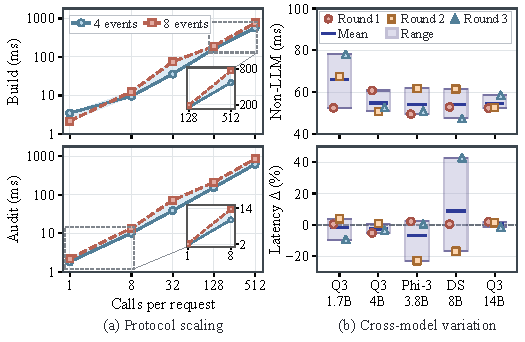
\includegraphics[width=\columnwidth]{b3_b4_scalability_variability.pdf}
  \caption{Protocol scalability and cross-model variability.
  (a) CPU construction (top) and audit (bottom) with four or eight events per call,
  sharing the call-count axis;
  shaded envelopes span those two configurations, with one measurement per point.
  Both axes in (a) are logarithmic;
  model inference and persistence are excluded.
  Linear-scale insets show 128--512 calls for construction and 1--8 calls for audit.
  (b) TokenProv online non-LLM time (top) and request latency change relative to Vanilla
  within the same round (bottom), sharing the model axis. In (b), shading spans the minimum and maximum of
  three round observations per model; markers show the individual rounds and
  dark horizontal bars show their arithmetic mean. Shading is not a confidence interval.
  Q3 denotes Qwen3; DS denotes DeepSeek-R1-Distill-Llama.}
  \label{fig:b3-b4-performance}
  \label{fig:b3-protocol-scalability}
\end{figure}

% B3: Fig.~\ref{fig:b3-b4-performance}(a).
% B4: Fig.~\ref{fig:b3-b4-performance}(b).
% Additional concurrency measurements appear in Appendix~\ref{app:b3-concurrency}.

% In the existing appendix, after \appendices:
% \section{Additional Scalability Measurements}
\label{app:b3-scalability}
\label{app:b3-concurrency}

\noindent\textbf{Protocol scaling.}
Table~\ref{tab:b3-protocol-scaling} reports the ten CPU protocol configurations
underlying the scalability curves: five call counts and two lifecycle-event
densities. Construction includes in-memory protocol generation and identity
initialization; audit checks the resulting signature-profile transcript.
Model inference, evidence persistence, ledger I/O, and proof generation are excluded.
Each configuration is measured once. The shaded envelopes in the main figure
therefore span configurations, rather than repeated-run uncertainty.
At 512 calls and 4,096 events, construction and audit take 764.82 and 864.69\,ms,
respectively.
\begin{table*}[!t]
\centering
\caption{Protocol construction and audit costs (one measurement per configuration).}
\label{tab:b3-protocol-scaling}
\footnotesize
\renewcommand{\arraystretch}{1.10}
\begin{tabular*}{\textwidth}{@{\hspace{4pt}}c@{\extracolsep{\fill}}cccc@{\hspace{4pt}}}
\toprule
\textbf{Calls/request} & \multicolumn{2}{c}{\textbf{4 events/call}} & \multicolumn{2}{c}{\textbf{8 events/call}} \\
\cmidrule(lr){2-3}\cmidrule(lr){4-5}
 & \textbf{Build (ms)} & \textbf{Audit (ms)} & \textbf{Build (ms)} & \textbf{Audit (ms)} \\
\midrule
1 & 3.48 & 1.82 & 2.16 & 2.22 \\
8 & 9.52 & 10.18 & 12.59 & 13.76 \\
32 & 35.94 & 38.87 & 74.94 & 71.81 \\
128 & 160.79 & 154.50 & 190.25 & 212.52 \\
512 & 566.98 & 620.65 & 764.82 & 864.69 \\
\bottomrule
\end{tabular*}
\end{table*}


\noindent\textbf{Serving concurrency.}
Table~\ref{tab:b3-concurrency} reports the original Qwen3-1.7B concurrency
measurements. Each scheme uses one measured round per configuration, with 16
requests at concurrency 1 and 128 at concurrency 8 and 32; warmups are excluded.
The concurrency-8 entries are the original round, rather than the later
three-round averages; these observations are reused in the cross-model cohort.
Each request comprises eight sequential calls, with
2,048 input tokens per call and an output limit of 256 tokens.
Latency is mean request processing time, excluding waiting for a worker slot.
Request and output throughput
are completed requests and generated tokens, respectively, divided by batch wall time.
Online non-LLM time is $T_{\mathrm{online}}-T_{\mathrm{llm}}$, where
$T_{\mathrm{llm}}$ accumulates model-service HTTP wall time.
Actual output length is included because the realized generation workload differs
across concurrency settings; request throughput alone does not isolate concurrency.
% Requires booktabs and xcolor with the table option (or colortbl).
\begin{table*}[!t]
\centering
\caption{Concurrency measurements for Qwen3-1.7B (one original round per configuration).}
\label{tab:b3-concurrency}
\footnotesize
\renewcommand{\arraystretch}{1.10}
\begin{tabular*}{\textwidth}{@{\hspace{4pt}}l@{\extracolsep{\fill}}cccccc@{\hspace{4pt}}}
\toprule
\textbf{Scheme} & \textbf{Requests} & \shortstack{\textbf{Latency}\\\textbf{(s)}} & \shortstack{\textbf{Throughput}\\\textbf{(req/s)}} & \shortstack{\textbf{Output rate}\\\textbf{(tokens/s)}} & \shortstack{\textbf{Online non-LLM}\\\textbf{(ms)}} & \shortstack{\textbf{Output length}\\\textbf{(tokens/call)}} \\
\midrule
\rowcolor{gray!12}
\multicolumn{7}{l}{\textbf{Concurrency 1}} \\
Vanilla & 16 & 6.893 & 0.145 & 65.51 & 1.18 & 56.45 \\
SignedLog & 16 & 6.995 & 0.143 & 64.56 & 3.57 & 56.45 \\
SignedLog+ & 16 & 6.999 & 0.143 & 64.51 & 14.03 & 56.45 \\
\textbf{\textsc{TokenProv}} & 16 & 7.033 & 0.142 & 64.20 & 13.33 & 56.45 \\
\midrule
\rowcolor{gray!12}
\multicolumn{7}{l}{\textbf{Concurrency 8}} \\
Vanilla & 128 & 11.365 & 0.703 & 192.49 & 1.30 & 34.24 \\
SignedLog & 128 & 14.719 & 0.543 & 147.35 & 10.80 & 33.95 \\
SignedLog+ & 128 & 14.997 & 0.529 & 144.64 & 58.24 & 34.16 \\
\textbf{\textsc{TokenProv}} & 128 & 11.409 & 0.700 & 191.68 & 52.46 & 34.23 \\
\midrule
\rowcolor{gray!12}
\multicolumn{7}{l}{\textbf{Concurrency 32}} \\
Vanilla & 128 & 67.262 & 0.472 & 245.10 & 1.00 & 64.91 \\
SignedLog & 128 & 89.193 & 0.356 & 184.74 & 11.17 & 64.91 \\
SignedLog+ & 128 & 72.323 & 0.438 & 227.59 & 86.04 & 64.91 \\
\textbf{\textsc{TokenProv}} & 128 & 59.350 & 0.535 & 277.84 & 85.01 & 64.90 \\
\bottomrule
\end{tabular*}
\end{table*}


